% =============================================================================
% Project : THE_PHILOSOPHY_OF_VIABILITY
% Book    : Book I — Ontology of Viability
% Book ID : VS.B01
%
% File    : 2_MAINMATTER/PART_I_IDENTITY_AND_MANIFESTATION/
%           CHAPTER_03_UNITY_AND_PLURALITY/sections/
%           section_04_plurality_of_identities.tex
%
% Section : Chapter 03, Section 04
% Title   : Plurality of Identities
%
% Purpose :
%   To examine the ontological possibility of more than one identity
%   within an existent or a broader configuration, while distinguishing
%   identity plurality from multiplicity of manifestations, components,
%   relations, sources, and aggregates.
%
% =============================================================================

\section{Plurality of Identities}
\label{sec:plurality-of-identities}

% -----------------------------------------------------------------------------
\subsection{The Ontological Question of Multiple Identities}

The possibility of plurality of identities raises a question
that cannot be resolved by counting the distinguishable elements
within an existent. The presence of several components,
manifestations, determinations, or relations does not by itself
establish that more than one identity is involved. Equally,
the consideration of an existent as one does not establish
that its identity is necessarily singular in every relevant
ontological respect.

The question is therefore more specific than the general
question of multiplicity. It concerns whether identity itself
may be plural within a given existent or configuration, and,
if so, under what ontological conditions such plurality may
be attributed.

This inquiry must remain open in both directions. It must
not assume that every existent necessarily possesses exactly
one identity. Nor may it assume that every complex existent
contains several identities merely because it exhibits
internal differentiation.

The task of this section is not to settle every possible
configuration in advance. It is to identify the distinctions
and requirements that an adequate account of identity plurality
must satisfy.

% -----------------------------------------------------------------------------
\subsection{Identity Plurality and Manifestational Multiplicity}

Plurality of manifestations and plurality of identities
are not equivalent claims.

An existent may manifest through several forms, states,
configurations, or modes. These manifestations may differ
in their properties and conditions while remaining related
to one identity. This possibility, however, does not establish
that all manifestational multiplicity must belong to one
identity.

The converse also requires care. A single manifestation,
considered at a particular level or under a particular
description, does not establish that only one identity
is involved in the relevant ontological configuration.

Accordingly, neither of the following inferences is
sufficient:

\[
\text{Plurality of Manifestations}
\not\Rightarrow
\text{Plurality of Identities}
\]

\[
\text{Unity of Manifestation}
\not\Rightarrow
\text{Unity of Identity}
\]

The distinction is not intended to separate manifestation
from identity as unrelated matters. Manifestation may be
ontologically relevant to the determination or expression
of identity. What is rejected is the assumption that a
numerical correspondence between manifestations and
identities can be established without further argument.

A plurality of manifestations may therefore be compatible
with different identity configurations. Whether a particular
case involves one identity, several identities, or an
unresolved relation among identities requires an independent
ontological examination.

% -----------------------------------------------------------------------------
\subsection{Identity Plurality and Component Multiplicity}

The plurality of components presents a related but distinct
problem. An existent may include several components that
differ materially, structurally, or relationally. Their
organization may constitute a composition or an aggregate,
but the number of components does not determine the number
of identities involved.

A component may be distinguishable within a composition
without thereby being established as an independently
distinct identity. Conversely, the integration of components
into an organized whole does not prove that the whole
involves only one identity or that no component has an
identity of its own.

The relevant questions must therefore be kept separate:

\begin{itemize}
    \item How many components are involved?
    \item What relations organize those components?
    \item What, if anything, is constituted as an aggregate
    or composition?
    \item To which components or configurations may identity
    be ontologically attributed?
    \item Are the identities so attributed distinct, unified,
    overlapping, or otherwise related?
\end{itemize}

These questions cannot be answered by a single count.
In particular, the attribution of identity to a component
and the attribution of identity to a composed existent
must not be treated as mutually exclusive alternatives
without justification.

% =============================================================================
% Project : THE_PHILOSOPHY_OF_VIABILITY
% Book    : Book I — Ontology of Viability
% Book ID : VS.B01
%
% File    : 4_ASSETS/tables/
%           VS.B01.P01.C03.S04.SS03.P003.TL01.identity_plurality_and_related_forms_of_multiplicity.tex
%
% Asset   : TL01 — Identity Plurality and Related Forms of Multiplicity
%
% Purpose :
%   To distinguish identity plurality from other forms of
%   ontological multiplicity and to prevent unsupported
%   inferences between them.
%
% =============================================================================

\begin{table}[htbp]
\centering
\caption{Identity Plurality and Related Forms of Multiplicity}
\label{tab:identity-plurality-and-related-multiplicity}

\small
\renewcommand{\arraystretch}{1.35}

\begin{tabular}{p{0.23\textwidth} p{0.34\textwidth} p{0.34\textwidth}}
\hline
\textbf{Form of multiplicity}
&
\textbf{What it concerns}
&
\textbf{What it does not establish by itself}
\\
\hline

Manifestational multiplicity
&
Several forms, states, configurations, or modes of manifestation.
&
That each manifestation constitutes a distinct identity.
\\

Component multiplicity
&
Several components within an existent, composition, or aggregate.
&
That each component has an independent identity, or that the whole has only one.
\\

Relational multiplicity
&
Several relations involving one or more relata.
&
The number of identities involved in the relational configuration.
\\

Source plurality
&
Several sources, origins, or grounds under a specified account.
&
A corresponding number of identities.
\\

Unity of source
&
A common source or origin related to several manifestations or configurations.
&
Unity or plurality of identity among those manifestations.
\\

Aggregate unity
&
The organization or grouping of elements as one aggregate under a criterion.
&
That the aggregate constitutes one identity or excludes several identities.
\\

Identity plurality
&
The attribution of more than one identity within a specified ontological scope.
&
A complete numerical structure or a universal rule governing all existents.
\\

\hline
\end{tabular}

\end{table}

% =============================================================================
% END OF ASSET TL01
% =============================================================================

The table distinguishes the principal kinds of multiplicity
relevant to this inquiry. Its purpose is not to provide
a complete classification of every possible ontological
configuration, but to prevent conclusions about identity
from being inferred directly from counts made at other
levels.

% -----------------------------------------------------------------------------
\subsection{Identity Plurality and Relational Multiplicity}

An existent may participate in several relations, and a
configuration may connect multiple relata through different
relational determinations. Such relational multiplicity
does not by itself establish plurality of identities.

Several relations may concern one identity under different
respects. Alternatively, relations may connect several
identities, or may belong to a configuration whose identity
structure has not yet been determined.

The number of relations is therefore not a measure of the
number of identities. Nor does the unity of a relational
subject establish that every relata or every element of
the broader configuration belongs to that same identity.

The ontological relevance of a relation to identity must
be specified. A relation may presuppose already distinguishable
identities, contribute to the determination of an identity,
connect identities without constituting them, or participate
in a more complex configuration. These possibilities must
not be collapsed into one general claim about relational
multiplicity.

Consequently, the analysis of identity plurality requires
attention not only to the relata and their relations, but
also to the ontological status attributed to each term
of the relation.

% -----------------------------------------------------------------------------
\subsection{Why Unity of Source Does Not Decide Identity Number}

The preceding section distinguished unity of source from
unity of identity. That distinction has a direct consequence
for the present inquiry: a common source cannot, by itself,
settle whether the manifestations or configurations related
to it involve one identity or several.

A common origin may establish a relation of derivation,
production, grounding, or another form of source-dependence.
The precise character of that relation must be examined
in each case. None of these descriptions, taken alone,
establishes identity unity.

Likewise, the attribution of several manifestations or
products to a common source does not prove that they
constitute several identities. The source relation settles
neither identity unity nor identity plurality.

The following distinction is therefore essential:

\[
\text{Common Source}
\not\Rightarrow
\begin{cases}
\text{One Identity},\\
\text{Multiple Identities}.
\end{cases}
\]

Any conclusion concerning identity must depend on further
ontological grounds. The source relation may be relevant
to those grounds, but its relevance cannot be substituted
for an account of identity itself.

% -----------------------------------------------------------------------------
\subsection{Identity Plurality Within a Unified Aggregate}

The unity of an aggregate also leaves the question of
identity plurality unresolved.

An aggregate may be unified according to a criterion
of grouping, organization, composition, or relation.
Such unity concerns the aggregate under the respect
specified by that criterion. It does not automatically
determine the identity status of the aggregate, its
components, or the broader configuration in which it
participates.

A unified aggregate may involve several identities.
It may also be considered as an aggregate without any
conclusion yet being established about whether it
constitutes an identity in its own right. These are
distinct possibilities, and neither should be treated
as universally applicable.

Similarly, the plurality of components within an aggregate
does not establish a plurality of identities among those
components. The aggregate relation and the identity
relations must be examined independently, even where
they intersect.

% =============================================================================
% Project : THE_PHILOSOPHY_OF_VIABILITY
% Book    : Book I — Ontology of Viability
% Book ID : VS.B01
%
% File    : 4_ASSETS/diagrams/
%           VS.B01.P01.C03.S04.SS06.P004.DG01.identity_plurality_across_ontological_levels.tex
%
% Asset   : DG01 — Identity Plurality Across Ontological Levels
%
% Purpose :
%   To display distinct levels at which unity and plurality
%   may be asserted, without implying a necessary hierarchy
%   or numerical correspondence among them.
%
% Requires (preamble):
%   \usepackage{tikz}
%   \usetikzlibrary{positioning, fit}
% =============================================================================

\begin{figure}[htbp]
    \centering

    \begin{tikzpicture}[
        font=\small,
        node distance=0.4cm,
        % --- base box ---
        box/.style={
            draw, rounded corners=3pt, align=center,
            inner sep=6pt, line width=0.7pt
        },
        % --- node roles ---
        levelbox/.style={box, text width=2.8cm, minimum height=1.4cm,
                         fill=blue!8, draw=blue!55!black},
        identitybox/.style={box, text width=6.4cm, minimum height=1.3cm,
                            fill=blue!16, draw=blue!55!black},
        % --- frames and labels ---
        vsgroup/.style={draw=black!45, dashed, rounded corners=5pt,
                        inner sep=8pt, line width=0.5pt},
        grouplabel/.style={font=\footnotesize\itshape, text=black!75,
                           align=left},
        elabel/.style={font=\footnotesize\itshape, text=black!75,
                       align=left, text width=4.6cm},
        % --- undirected link (no arrowheads: no priority, no entailment) ---
        vslink/.style={draw=black!55, dashed, line width=0.7pt}
    ]

    % ---------------------------------------------------------------
    % Row 1: three levels
    % ---------------------------------------------------------------
    \node[levelbox] (manifestation) {
        \textbf{Manifestation}\\[3pt]
        One or many forms
    };
    \node[levelbox, right=of manifestation] (components) {
        \textbf{Components}\\[3pt]
        One or many elements
    };
    \node[levelbox, right=of components] (relations) {
        \textbf{Relations}\\[3pt]
        One or many connections
    };

    % ---------------------------------------------------------------
    % Row 2: two levels, centred under the row above
    % ---------------------------------------------------------------
    \node[levelbox, below=of components, xshift=-1.8cm] (source) {
        \textbf{Source}\\[3pt]
        One or many grounds
    };
    \node[levelbox, below=of components, xshift=1.8cm] (aggregate) {
        \textbf{Aggregate}\\[3pt]
        Unity by a grouping criterion
    };

    % ---------------------------------------------------------------
    % Frame: five levels of equal rank
    % ---------------------------------------------------------------
    \node[vsgroup, fit=(manifestation)(components)(relations)
                       (source)(aggregate)] (levels) {};
    \node[grouplabel, anchor=south west] at (levels.north west) {
        Levels at which unity and plurality may be asserted
    };

    % ---------------------------------------------------------------
    % Identity (outside the frame)
    % ---------------------------------------------------------------
    \node[identitybox, below=1.1cm of levels] (identity) {
        \textbf{Identity}\\[3pt]
        Unity or plurality requiring identity-level grounds
    };

    \draw[vslink] (levels.south) -- (identity.north)
        node[elabel, midway, right=5pt] {
            possible relevance for inquiry
        };

    % ---------------------------------------------------------------
    % Analytical constraint
    % ---------------------------------------------------------------
    \node[below=0.7cm of identity, text width=10.5cm, align=center,
          font=\footnotesize\itshape] {
        \textbf{Analytical constraint:}
        A unity or plurality claim at one level does not determine
        the identity configuration at another level without
        additional ontological grounds. The connection indicates
        possible relevance for inquiry, not entailment, causation,
        or a fixed hierarchy.
    };

    \end{tikzpicture}

    \caption{Distinct ontological levels relevant to the analysis of
    identity plurality}
    \label{fig:identity-plurality-across-ontological-levels}
\end{figure}

% =============================================================================
% END OF ASSET DG01
% =============================================================================

The diagram represents different levels at which unity
and plurality may be considered. It does not depict a
necessary hierarchy, a causal sequence, or a one-to-one
correspondence. Its purpose is to show why a conclusion
drawn at one level cannot be transferred to another
without an additional argument.

% -----------------------------------------------------------------------------
\subsection{The Requirement of Identity Distinction}

To establish that more than one identity is involved,
it is necessary to explain what makes the identities
distinct as identities. Differences in appearance,
location, composition, function, or relation may provide
relevant evidence for an inquiry, but none of these
differences is automatically equivalent to identity
distinction.

Two configurations may differ in several determinations
while remaining related to one identity. Conversely,
two identities may share properties, structures, sources,
or relations without thereby becoming one identity.

Thus, neither similarity nor difference is sufficient
on its own to determine identity unity or plurality.
Similarity requires a specified respect of comparison;
difference requires an account of its ontological
significance. The question of identity cannot be settled
merely by describing the degree of resemblance or
dissimilarity between two configurations.

An adequate account must therefore distinguish at least
three questions:

\begin{enumerate}
    \item What differences are present between the
    configurations under consideration?
    \item Which of those differences are ontologically
    relevant to identity?
    \item What grounds warrant attributing distinct
    identities rather than different determinations
    or manifestations of one identity?
\end{enumerate}

The third question cannot be answered by presupposing
that every difference constitutes an identity boundary.
Nor can it be answered by assuming that shared
determinations necessarily erase identity distinction.

Identity distinction must be established at the level
of identity itself. It must not be reduced to numerical
difference between descriptions, observable forms,
or enumerated components.

% -----------------------------------------------------------------------------
\subsection{Boundaries, Overlap, and Relations Between Identities}

The possibility of several identities raises the question
of how their respective domains are distinguished.
However, identity boundaries must not be identified
without qualification with spatial, material, functional,
or structural boundaries.

Spatial separation may distinguish two existents under
a spatial respect, but it does not by itself provide
a complete account of their identities. Material continuity
may connect components or configurations without proving
that they belong to one identity. Structural integration
may establish an organized whole without excluding
identity distinctions within that whole.

Nor should identity plurality be assumed to consist
only of mutually isolated identities. If several identities
are involved in a configuration, they may stand in relations
of dependence, interaction, constitution, coordination,
or other forms of connection. The existence of such
relations does not automatically eliminate their distinction.

The possibility of overlap or nested organization also
requires careful treatment. A broader configuration may
include elements whose identity status differs from that
of the configuration considered as a whole. Whether
such a configuration involves one identity, several
identities, or another ontological arrangement cannot
be decided by importing ordinary spatial models of
containment.

% =============================================================================
% Project : THE_PHILOSOPHY_OF_VIABILITY
% Book    : Book I — Ontology of Viability
% Book ID : VS.B01
%
% File    : 4_ASSETS/illustrations/
%           VS.B01.P01.C03.S04.SS08.P003.IL01.multiple_identity_attributions_within_one_configuration.tex
%
% Asset   : IL01 — Multiple Identity Attributions Within One Configuration
%
% Purpose :
%   To provide an intuitive illustration of how several
%   distinguishable elements may participate in one broader
%   configuration while the identity status of the elements
%   and the configuration remains a separate question.
%
% =============================================================================

\begin{figure}[htbp]
\centering

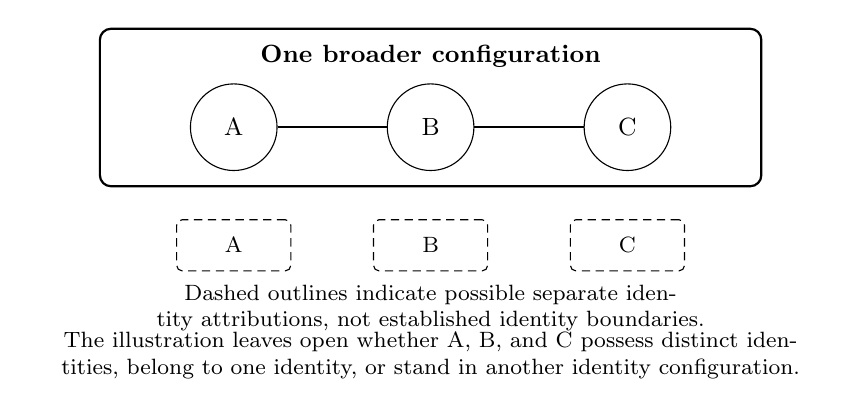
\begin{tikzpicture}[
    element/.style={
        circle,
        draw,
        minimum size=11mm,
        font=\small
    },
    possible/.style={
        draw,
        densely dashed,
        rounded corners=2pt,
        minimum width=1.45cm,
        minimum height=0.65cm,
        font=\footnotesize
    }
]

% Broader configuration
\draw[thick, rounded corners=4pt]
    (-4.2,1.0) rectangle (4.2,-1.0);

\node[font=\small\bfseries] at (0,0.65) {
    One broader configuration
};

% Elements within the configuration
\node[element] (a) at (-2.5,-0.25) {A};
\node[element] (b) at (0,-0.25) {B};
\node[element] (c) at (2.5,-0.25) {C};

\draw[thick] (a) -- (b);
\draw[thick] (b) -- (c);

% Possible identity attributions
\node[possible] at (-2.5,-1.75) {
    A
};

\node[possible] at (0,-1.75) {
    B
};

\node[possible] at (2.5,-1.75) {
    C
};

\node[
    align=center,
    text width=10cm,
    font=\footnotesize
] at (0,-2.55) {
    Dashed outlines indicate possible separate identity
    attributions, not established identity boundaries.
};

\node[
    align=center,
    text width=10cm,
    font=\footnotesize
] at (0,-3.15) {
    The illustration leaves open whether A, B, and C
    possess distinct identities, belong to one identity,
    or stand in another identity configuration.
};

\end{tikzpicture}

\caption{A unified configuration with identity attributions left open}
\label{fig:multiple-identity-attributions-within-one-configuration}

\end{figure}

% =============================================================================
% END OF ASSET IL01
% =============================================================================

The illustration provides a concrete way to consider
different possible attributions within one organized
configuration. It is illustrative rather than evidential:
it does not establish that the depicted elements possess
distinct identities, nor that the encompassing configuration
constitutes an additional identity. Those conclusions
would require independent ontological grounds.

% -----------------------------------------------------------------------------
\subsection{Plurality Without Premature Enumeration}

Even where identity plurality is established in a particular
case, its numerical structure requires further examination.
The recognition that more than one identity is involved
does not by itself determine the total number of identities,
their relations, or the principles by which they are
distinguished.

The identities involved need not be assumed to form
a collection of independent and mutually isolated units.
They may be related in ways that affect their constitution,
manifestation, or organization without necessarily
eliminating their distinction.

Likewise, the recognition of a broader configuration
does not automatically establish an additional identity
above or beyond the identities already distinguished.
A higher-order identity, if proposed, would require
its own ontological justification rather than being
inferred from the mere existence of a grouping or
composition.

For these reasons, identity plurality should not be
reduced to a numerical inventory made before the relevant
identity criteria have been clarified. Enumeration
presupposes that the units to be counted have already
been identified as identities. Where that prior
determination remains unsettled, a numerical conclusion
would merely restate the unresolved question.

% -----------------------------------------------------------------------------
\subsection{Conditions for a Responsible Attribution of Identity Plurality}

The preceding analysis indicates that an attribution
of identity plurality requires more than the observation
of multiplicity. At a minimum, an adequate account
must clarify the subject of the attribution, the respect
under which plurality is asserted, and the grounds
for distinguishing the identities involved.

It must also distinguish identity plurality from
manifestational, compositional, and relational multiplicity.
Where a common source or unified aggregate is relevant,
the account must explain precisely what follows from
that relation and what does not.

The requirements may be stated as follows:

\begin{enumerate}
    \item The entities or configurations to which identity
    is attributed must be specified.
    \item The respect and scope of the plurality claim
    must be made explicit.
    \item The grounds for distinguishing identities must
    be stated rather than inferred from difference alone.
    \item Relations among the identities must be examined
    without presuming that relation either eliminates
    or guarantees distinction.
    \item The attribution must not depend solely on the
    number of manifestations, components, relations,
    sources, or aggregates.
    \item The conclusion must remain proportionate to
    the grounds actually established.
\end{enumerate}

These requirements are methodological constraints on
ontological argument. They do not constitute a completed
definition of identity plurality, nor do they provide
a universal test that can be applied without regard
to the particular ontological problem.

Their function is to prevent unsupported transitions
from one kind of multiplicity to another and to make
explicit what an argument for identity plurality would
need to establish.

% -----------------------------------------------------------------------------
\subsection{Conclusion: Identity Plurality as an Open Ontological Problem}

Plurality of identities is a genuine ontological possibility
that cannot be excluded merely by appealing to the unity
of an existent, a common source, or a unified aggregate.
At the same time, it cannot be established merely by
counting components, manifestations, relations, or
differences between configurations.

The inquiry has therefore maintained the distinction
between identity plurality and other forms of multiplicity.
It has also shown that identity distinction requires
grounds that are relevant to identity itself. Similarity,
difference, spatial separation, material continuity,
structural integration, and relational connection may
be relevant to the analysis, but none independently
settles the question in every case.

No universal conclusion has been established here
that every existent possesses exactly one identity.
Nor has the universal attribution of multiple identities
been established. The number and organization of identities
must remain open wherever the relevant ontological
grounds have not been sufficiently determined.

The next section examines plurality and composition
more directly. It will consider the relation between
compositional organization and identity without assuming
that the plurality of components either entails or
excludes plurality of identities.

% =============================================================================
% END OF SECTION 04 OF CHAPTER 03
% =============================================================================